%!TeX root=../main.tex


% TODO: 
% * To make clearer in gen 8 change 'step' to 'sig' and test again (it is illustrative anyway)
% * Color code neurons better


\begin{figure}[!htb]        
\vskip -0.00in % useful knobs to optimize layout
    \centering        
    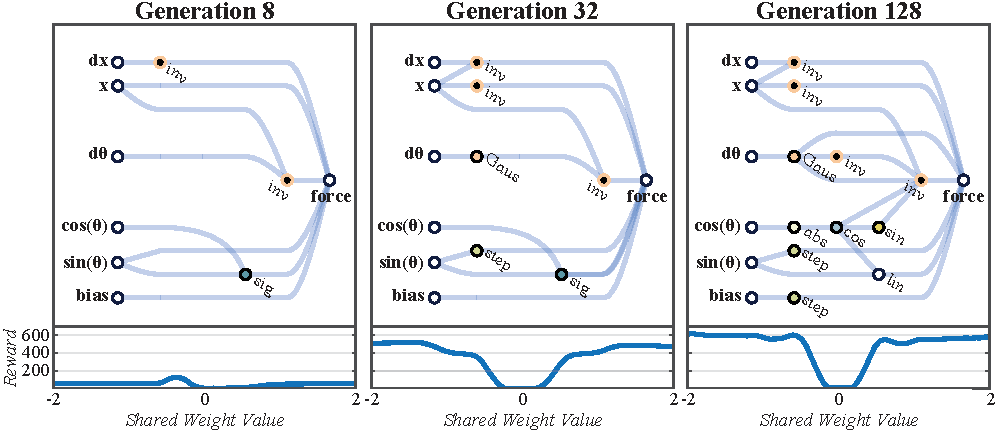
\includegraphics[width=1\textwidth]{img/swing.pdf}   
\vskip -0.05in % useful knobs to optimize layout
    \caption      
    {     
        \textit{Development of Weight Agnostic Neural Network Topologies Over Time}
        \newline
        \textit{Generation 8:} An early network which performs poorly with nearly all weights.
        \newline
        \textit{Generation 32:} Relationships between the position of the cart and velocity of the pole are established. The tension between these relationships produces both centering and swing-up behavior.
        \newline
        \textit{Generation 128:} Complexity is added to refine the balancing behavior of the elevated pole.
    }         
    \label{fig:swingNets}      
\vskip -0.05in % useful knobs to optimize layout
\end{figure}
